
\clearpage

\section{Anforderungs - und Mängelmanagement}
\label{bkm:Ref2018071701}

In diesem Kapitel wird das CUBE Anforderungs - und Mängelmanagement beschrieben.

\vspace{\baselineskip}

Das Modul 'Anforderungs - und Mängelmanagement' ist ein Hilfsmittel zur Erfassung und Verwaltung von technischen, baulichen, betrieblichen und organisatorischen Anforderungen auf allen Projektstufen. Der Workflow orientiert sich dabei an einem Statussystem, welches den Benutzer durch sämtliche Arbeitsschritte / Prozesse wie Anforderungen erfassen und validieren, Mängel aufnehmen und deren Behebung nachweisen u.a. führt. Mittels dem Modul 'Anforderungs- und Mängelmanagement' haben Sie jederzeit den Überblick über eine Abnahme und wissen genau, welche Arbeiten noch erledigt oder nachgebessert werden müssen.

\vspace{\baselineskip}

\textbf{Hinweis zum Statussystem:} Das in diesem Handbuch verwendete Statussystem orientiert sich an einem Praxisbeispiel. Ein Statussystem wird in der Regel nach Absprache mit dem Kunden und dem Einsatzgebiet / den Gegebenheiten abgestimmt und eingeführt.

\vspace{\baselineskip}

Das Modul beinhaltet folgende 4 Kategorien:

\vspace{\baselineskip}

\begin{compactitem}
	\item Anforderungen
	\item Arbeitspakete
	\item Mängel (Vorbehalte)
	\item Pendenzen
\end{compactitem}

\vspace{\baselineskip}

\textbf{Anforderungen:} Zuerst werden die Anforderungen erfasst, welche im Zusammenhang mit dem Projekt, den Vorbereitungen oder Umsystemen stehen. \\

\textbf{Arbeitspakete:} Sie beschreiben Arbeitsschritte eines Projekts oder fassen gewisse Arbeiten zusammen, welche bspw. einen Auftragsnehmer betreffen. \\

\textbf{Mängel (Vorbehalte):} Bezeichnen die Mängel an Projektarbeiten, welche noch einer Korrektur oder Besserung bedürfen. Sie können mit Pendenzen oder Arbeitspaketen verknüpft werden. Die Mängel beziehen sich jeweils auf eine Anforderung. Mängel erhalten einen Status, welcher den Projektzustand wiedergibt (Beispielsweise: Freigegeben und Abgeschlossen). Das Statussystem kann kundenspezifisch konfiguriert werden. \\

\textbf{Pendenzen:} Die Pendenzen entsprechen den Pendenzen des Sitzungswesens und können Bestandteil eines Mangels sein. 

\pagebreak

\subsection{Anforderungsübersicht}

Unter Übersicht oder Anforderungsübersicht finden Sie auf einen Blick die 'Anforderungsstatistik'. Diese zeigt Ihnen den Anteil / Fortschritt eines jeden Status an.

\begin{figure}[H]
\center{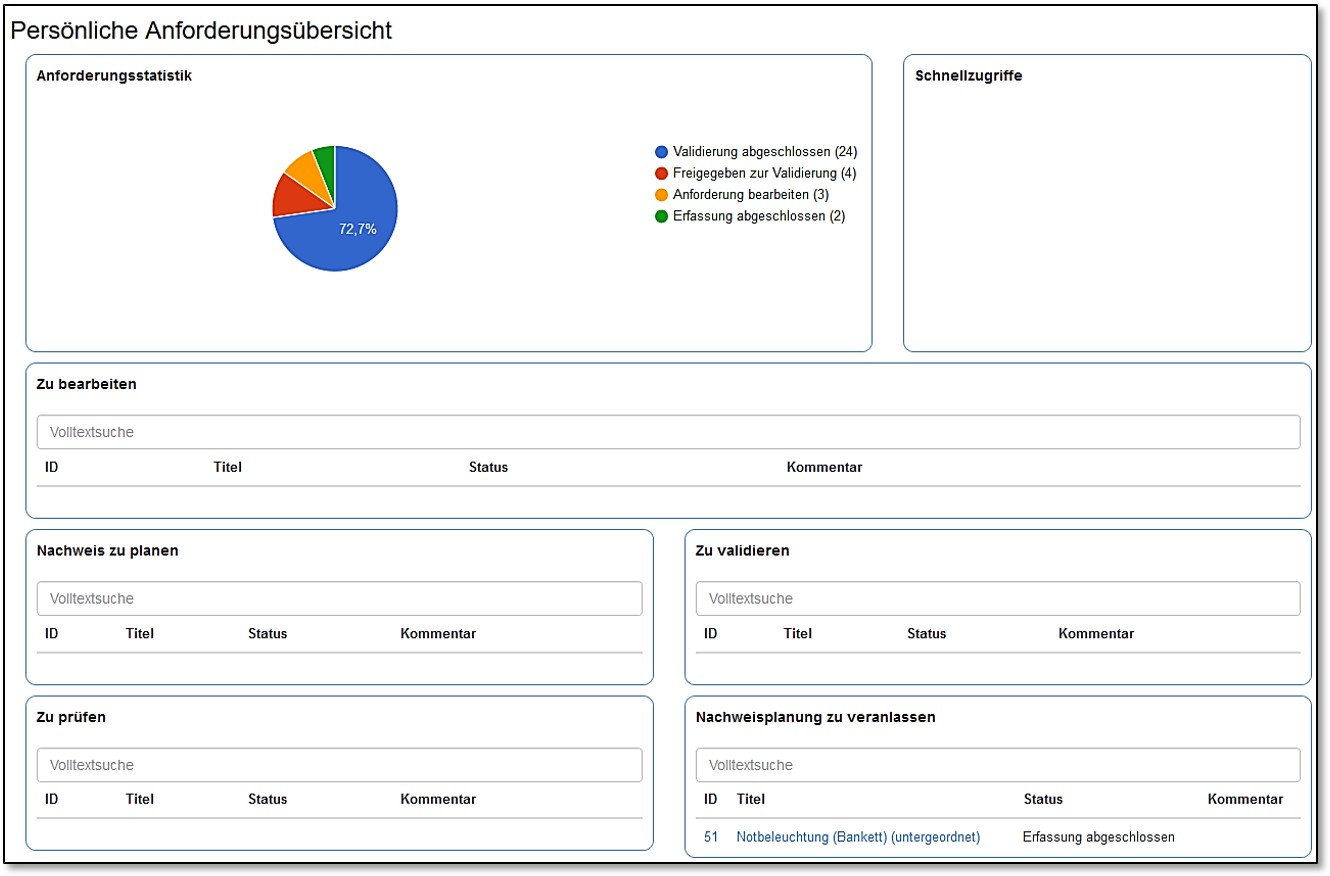
\includegraphics[width=1\linewidth]{../chapters/06_Anf-Maengelmanagement/pictures/amm_Dashboard.jpg}}
\caption{Die Anforderungsstatistik}
% \label{fig:speciation}
\end{figure}

\textbf{Anforderungsstatistik}
Grafisch dargestellt sehen Sie die Aufteilung in Prozent sämtlicher Anforderungen nach Status. In Klammern hinter der Legende sehen Sie wie viele Anforderungen einem Status zugeordnet sind. \\

\textbf{Schnellzugriffe}
Durch die 'Schnellzugriffe' können Sie direkt auf gefilterte Sets von Anforderungen, Dokumenten und Pendenzen zugreifen. \\

\textbf{Übersicht über Status}
Abhängig von der Rolle, die ein Mitarbeiter inne hat, werden ihm Kacheln angezeigt, welche seine nächsten Schritte festhalten. In diesen Kacheln kann er dann direkt auf die entsprechenden Anforderungen klicken und die weitere Bearbeitung vornehmen.

\pagebreak

\subsection{Anforderungen: Einstieg und Anwendung}

\begin{wrapfigure}[3]{l}{6.5cm}   % [x] Wie manche Zeile soll sich um die Grafik "brechen"
  \vspace{-30pt}      % Grundwert war 20; mit 30 schön oben beim Text ausgerichtet
  \begin{center}
    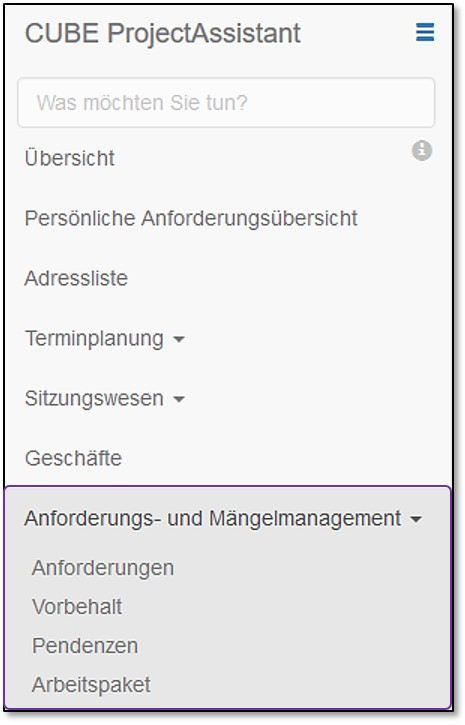
\includegraphics[width=1\linewidth]{../chapters/06_Anf-Maengelmanagement/pictures/amm_Menue.jpg}
  \end{center}
  \vspace{-20pt}
  \caption{Das Anforderungs- und Mängelmanagement verwenden}
  \vspace{-10pt}
\end{wrapfigure}

Wählen Sie im Menü links den Punkt 'Anforderungs- und Mängelmanagement' und dann den Unterpunkt 'Anforderungen'.

% \pagebreak
\vspace{10.5cm}

Sie sehen die Übersicht der Anforderungen. Die gewohnte Arbeitsweise von CUBE PA können Sie auch hier anwenden. (Volltextsuche, Spalten filtern und sortieren, sowie Spalten ein- und ausblenden 
\includegraphics[height=12pt]{/Icons/SpaltenEinst.jpg} etc.).

\begin{figure}[H]
\center{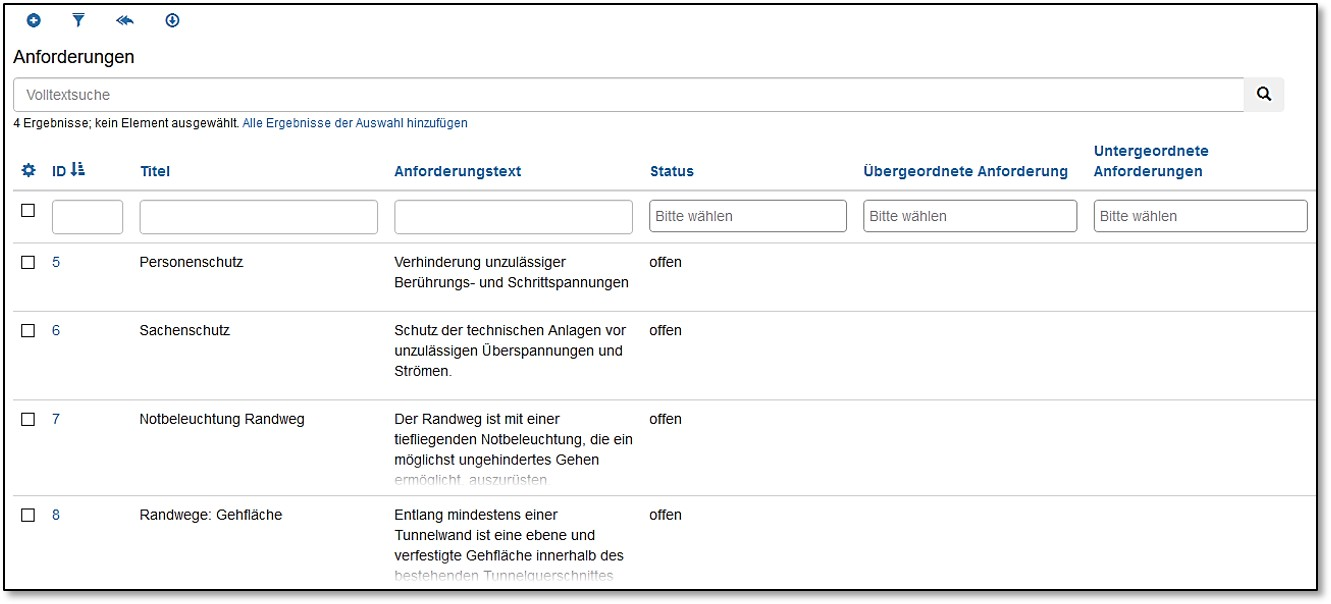
\includegraphics[width=1\linewidth]{../chapters/06_Anf-Maengelmanagement/pictures/amm_Anf_Uebersicht.jpg}}
\caption{Die Anforderungsübersicht}
% \label{fig:speciation}
\end{figure}

\subsection{Benutzerrollen:} 
Benutzer können grundsätzlich in drei Rollen eingeteilt werden: Ersteller (Autor Anforderungen), Validierer und Teilprojektleiter Validierung (TPL Validierung). Diese Benutzerrollen haben zentrale Aufgaben im RAMS- und Validierungsprozess.

\subsubsection{Ersteller (Autor Anforderungen):} 
Der Ersteller verfasst und bearbeitet Anforderungen (Siehe Kapitel \ref{bkm:Ref2018071810}). Er prüft die Anforderungen auf Vollständigkeit und schaltet den Status auf 'Anforderungen erfasst' weiter. Wird der Status einer Anforderung zurückgesetzt, kann er diese erneut bearbeiten, splitten oder gruppieren. \\
Ausserhalb der Bearbeitung von Anforderungen hat der Ersteller nur eine Leseberechtigung. Jeder Ersteller kann jede Anforderung bearbeiten. Dies ermöglicht eine grosse Flexibilität beim Wechsel des Erstellers. Eine gleichzeitige Bearbeitung eines Datensatzes (derselben Anforderung) durch einen zweiten Ersteller wird verhindert. Der zweite Ersteller wird darüber informiert, wer momentan den Anforderungseintrag bearbeitet. 

\subsubsection{Validierer:} 
Nach dem Statuswechsel von 'Erfassung abgeschlossen' zu 'Nachweisplanung' führt der Validierer die Planung der Nachweisführung durch (siehe Kapitel \ref{bkm:Ref2018071811}). Dabei erfasst er einen Eintrag zur Nachweisplanung in der Rubrik 'Validierung der Anforderung (Planung)', welche aufzeigt, wie er die Anforderungen nachweisen bzw. validieren will. Ist die Planung abgeschlossen setzt er den Status von 'Nachweisplanung' zu 'Überprüfung der Nachweisplanung'. \\

Ist die Planung in Ordnung wird die Validierung freigegeben und der Validierer kann die Nachweise für die Validierung selbst durchführen oder über Drittpersonen einholen. Sind alle notwendigen Nachweise vorhanden und damit die Nachweise vollständig, erfasst er einen Eintrag in der Rubrik 'Validierung der Anforderungen (Durchführung)'. Ist dies erfolgt, kann der Validierer den Status von 'Freigegeben zur Validierung' zu 'Überprüfung der Validierung' weiterschalten (siehe Kapitel \ref{bkm:Ref2018071812}). 
Ausserhalb der Bearbeitung von Anforderung hat der Validierer nur eine Leseberechtigung. Jeder Validierer kann jede Nachweisplanung und -durchführung bearbeiten. Dies ermöglicht eine grosse Flexibilität beim Wechsel des Validierers. Eine gleichzeitige Bearbeitung desselben Nachweises durch zwei Validierer wird verhindert. Der zweite Validierer wird darüber informiert, wer momentan den Nachweiseintrag bearbeitet.

\subsubsection{TPL Validierung:}

Der Teilprojektleiter Validierung hat die Aufgabe den RAMS- und Validierungsprozess zu überprüfen und entsprechend den Status im Prozess weiter zu schalten. Es ist daher davon abzusehen, dass der TPL Validierung gleichzeitig auch Autor (Ersteller) oder Validierer ist. Hat der Ersteller eine Anforderung erfasst, überprüft der TPL Validierung die Anforderung und schaltet den Status weiter zu 'Erfassung abgeschlossen' oder im Fall einer fehlerhaften Anforderung zurück auf den Status 'Anforderung bearbeiten'. Die Kontrolle über den Status wechselt dann wieder zum Ersteller. \\

Bei beiden Überprüfungen (Nachweisplanung und Validierung) muss der TPL Validierung entscheiden, ob der Sachverhalt zutrifft und die Informationen und Dokumente vollständig vorhanden sind. Bei einer fehlerhaften oder unvollständigen Aufgabenerfüllung kann er den Status jeweils zurücksetzen und gibt die Kontrolle über den Status wieder an den Validierer ab. Iterationen können mehrmals durchlaufen werden, bis der Prozess fortgeführt werden kann. \\

Der Endzustand beschliesst die Validierung mit erfüllten oder nicht erfüllten Anforderungen. Der TPL Validierung muss dann je nach Erfüllungsgrad weitere Prüfungen von Massnahmen in die Wege leiten.

\subsubsection{Passive Benutzer bezüglich Inhalt und Prozesse:} 

Unter passiven Benutzern versteht man Benutzerrollen, welche keinen aktiven Einfluss auf die Prozesse haben. Dies können einerseits 'Leser' sein, welche lediglich Leserechte auf alle Einträge haben. Andererseits können dies 'Administratoren' sein, welche für die Vergabe von Zugriffsrechten und die Zuteilung von Benutzerrollen verantwortlich sind. Der Administrator sollte nur in Notfällen direkt in die Prozesssteuerung eingreifen müssen.

\subsection{Prozesse und Abläufe}

Die Prozesse und Abläufe werden nachfolgend anhand der Status beschrieben, welche ein einzelner Anforderungseintrag durchläuft. 

\vspace{\baselineskip}

\textbf{Hinweis:} Das Statussystem / der Prozessablauf ist projekt- / kundenspezifisch und wird demnach nach Absprache mit dem Kunden konfiguriert. Diese Anleitung orientiert sich an einem Praxisbeispiel, entsprechend sind Abweichungen möglich.

\vspace{\baselineskip}

Eine Besonderheit des Anforderungs- und Mängelmanagements ist die grafische Weiterschaltung des Statussystems. Mit farbigen Buttons wird dem Benutzer immer der nächste Schritt oder die Rückgabe an vorhergehende Stelle angezeigt. Mit wenigen Klicks wird die Anforderung durch den Prozess geführt.

\begin{figure}[H]
\center{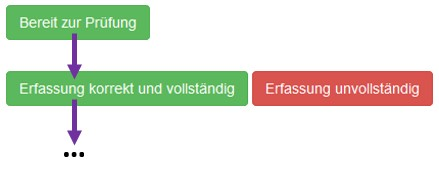
\includegraphics[width=.45\linewidth]{../chapters/06_Anf-Maengelmanagement/pictures/amm_grafStatus.jpg}}
% \caption{Anforderung erstellen oder bearbeiten}
% \label{fig:speciation}
\end{figure}

\subsection{Anforderungen erstellen und bearbeiten}
\label{bkm:Ref2018071810}

\begin{figure}[H]
\center{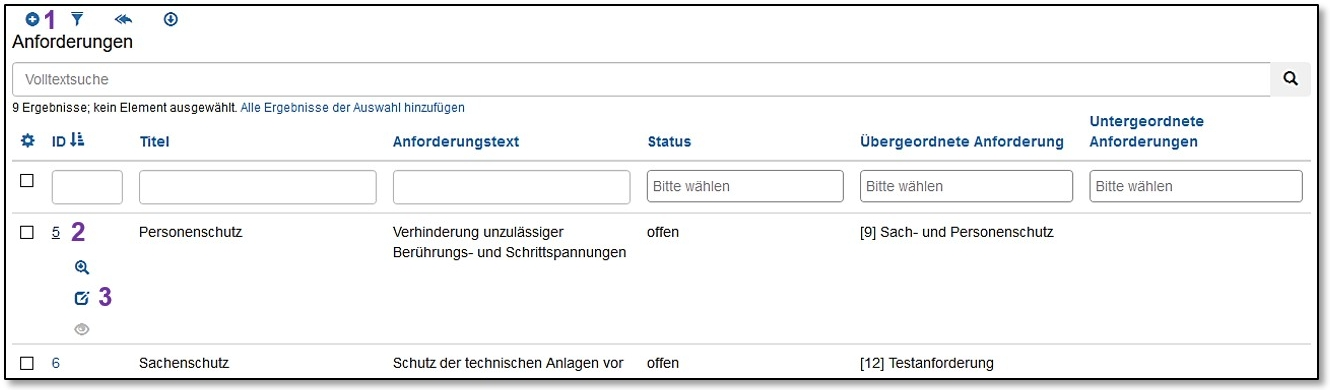
\includegraphics[width=1\linewidth]{../chapters/06_Anf-Maengelmanagement/pictures/amm_AnfBearbeiten.jpg}}
\caption{Anforderung erstellen oder bearbeiten}
% \label{fig:speciation}
\end{figure}

\subsubsection{Neue Anforderung erstellen}

Mit Klick auf das Plussymbol (
\includegraphics[height=12pt]{/Icons/Plussymbol.jpg}) \col{(1)} wird eine neue Anforderung erstellt. Nun müssen alle Pflichtfelder ausgefüllt und der Eintrag durch die blaue Schaltfläche 'Erstellen' gespeichert werden. 

\subsubsection{Bestehende Anforderung bearbeiten}

Eine bestehende Anforderung wird wie folgt bearbeitet: In der Anforderungsübersicht die gewünschte Anforderung suchen und mit Klick auf die 'ID'-Nummer \col{(2)} öffnen sich weitere Optionen. Wählen Sie das Bearbeiten-Symbol (
\includegraphics[height=12pt]{/Icons/bearbeiten.jpg}) \col{(3)}. Nun erscheinen die bisherigen Angaben in einer Maske. Die Maske zum Bearbeiten von Anforderungen beinhaltet einige Pflichtfelder, welche mit einem Stern (*) markiert sind. Diese müssen zwingend ausgefüllt oder ausgewählt werden, falls dies beim Erstellen noch nicht erfolgt ist. Für gewisse Felder sind mehrere Auswahlen möglich. Nach dem Erfassen der Anforderung müssen die Änderungen übernommen werden, damit sie in der Datenbank gespeichert werden. Die entsprechende blaue Schaltfläche 'Übernehmen' befindet sich unten an der Maske oder alternativ oben in der Mitte der Leiste. Wollen Sie nach dem Speichern gleich zur Übersicht zurückkehren, klicken Sie auf 
\includegraphics[height=12pt]{/Icons/ueb_schliessen.png} oben in der Mitte des Bildschirms. \\

\vspace{\baselineskip}

\textbf{Hinweis:} Falls bei den Optionen einer Anforderung das Bearbeiten-Symbol (
\includegraphics[height=12pt]{/Icons/bearbeiten.jpg}) fehlt, besitzen Sie nur Leserechte und können die Anforderung nicht ändern.

%\clearpage
\vspace{\baselineskip}

\textbf{Mehrere Anforderungen bearbeiten}

Um mehrere Anforderungen zu überarbeiten, können diese mit Häkchen (
\includegraphics[height=12pt]{/Icons/checkbox_markiert.jpg}) ausgewählt werden. Danach ist es möglich mit der Schaltfläche 'Serienbearbeitung' (
\includegraphics[height=12pt]{/Icons/A_Serienbearbeitung.jpg}) in der Menüleiste die einzelnen Anforderungen nacheinander zu bearbeiten und jeweils mit dem Button 
\includegraphics[height=12pt]{/Icons/speichern_weiter.jpg} \col{(2)} zur nächsten Anforderung zu springen ohne diese erneut auswählen zu müssen. Mit dem 
\includegraphics[height=12pt]{/Icons/Abbrechen_r.jpg}-Symbol \col{(1)} können Sie die Maske ohne die Daten zu speichern wieder verlassen. \\

\begin{figure}[H]
\center{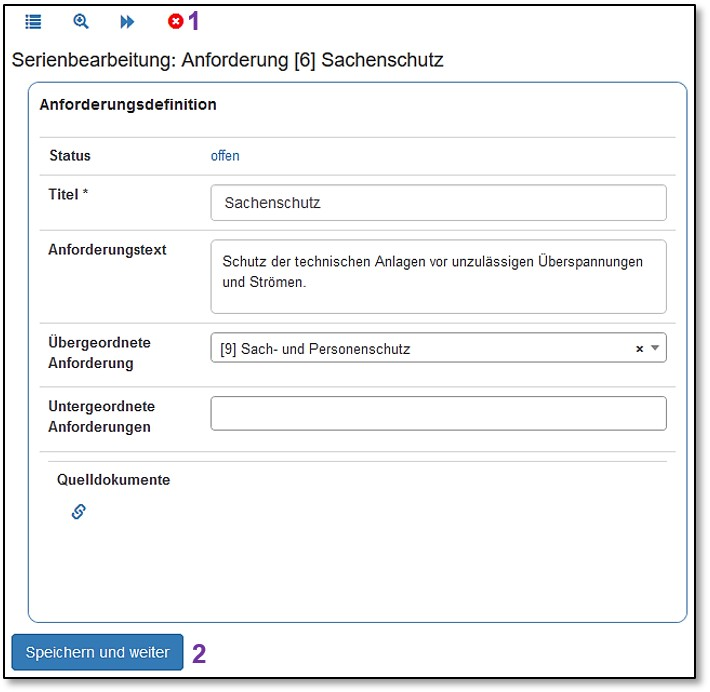
\includegraphics[width=0.5\linewidth]{../chapters/06_Anf-Maengelmanagement/pictures/amm_mAnfBearbeiten.jpg}}
\caption{Anforderung erstellen oder bearbeiten}
% \label{fig:speciation}
\end{figure}

Nach dem Erstellen und während dem Bearbeiten kann jeder Anforderung ein Quelldokument angehängt werden. Dieses Dokument muss vorher in der Dokumentenablage erfasst worden sein (Siehe Kapitel \ref{bkm:Ref442863508}). 

\subsubsection{Anforderungen gruppieren}

Der TPL Validierung hat die Möglichkeit für mehrere Anforderungen, welche z.B. thematisch oder organisatorisch zusammengehören, eine neue übergeordnete Anforderung zu erstellen. Diese Funktion steht nur für Anforderungen zur Verfügung, welche sich aktuell im Status 'Erfassung abgeschlossen' befinden. Sowohl die existierenden (Unter-)Anforderungen wie auch die neu erstellte übergeordnete Anforderung durchlaufen anschliessend den normalen Lebenszyklus gemäss Statuskonfiguration. Bevor die übergeordnete Anforderung in den abschliessenden Status 'Validierung abgeschlossen' verschoben werden kann, wird automatisch geprüft, ob die Validierung aller untergeordneten Anforderungen bereits abgeschlossen ist. Andernfalls erscheint eine Warnung. \\

\textbf{Vorgehen:}
Mehrere bestehende Anforderungen können in der Anforderungsübersicht ausgewählt werden (mittels Checkbox 
\includegraphics[height=12pt]{/Icons/checkbox_markiert.jpg}). Durch Klicken der Schaltfläche 'Gruppieren' 
\includegraphics[height=12pt]{/Icons/A_Gruppieren.jpg} wird die Eingabemaske zur Erstellung einer neuen Anforderung geöffnet, wobei die zuvor gewählten Anforderungen als untergeordnete Anforderungen ('Kinder') vorausgewählt werden. Ebenfalls werden Mehrfachauswahlfelder vorausgefüllt (Summe aller Auswahlen der 'Kinder') und ggf. Einfachauswahlfelder ausgefüllt (nur falls Auswahl bei den 'Kindern' identisch ist).
Nach erfolgreichem Gruppieren können die hierarchischen Verknüpfungen der Anforderungen in einem Baum dargestellt werden. Nach Auswahl einer Anforderung erfolgt dies über die Baumschaltfläche (
\includegraphics[height=12pt]{/Icons/A_Anforderungsbaum.jpg}) in der Titelleiste.

\subsubsection{Anforderungen splitten}

Die Anforderungsautoren haben die Möglichkeit, einzelne Anforderungen in mehrere An-forderungen aufzuteilen. Dabei wird bei jedem Splitting-Vorgang eine neue Anforderung erfasst, die der bereits existierenden Anforderung untergeordnet und standardmässig mit demselben Inhalt vorausgefüllt ist. Analog zum beschriebenen Verhalten beim Gruppieren von Anforderungen durchlaufen anschliessend alle existierenden und neuen Anforderungen den normalen Lebenszyklus. Für die übergeordneten Anforderungen wird ebenfalls (unabhängig davon, ob sie durch Gruppierung oder Splitting entstanden sind) vor dem Abschluss geprüft, ob alle untergeordneten Anforderungen abschliessend validiert sind. \\

\textbf{Vorgehen:}
Durch Auswahl einer bestehenden Anforderung (mittels Checkbox 
\includegraphics[height=12pt]{/Icons/checkbox_markiert.jpg}) und Klicken der Schaltfläche 'Splitten'  (
\includegraphics[height=12pt]{/Icons/A_Splitten.jpg}) wird die Eingabemaske zur Erstellung einer neuen Anforderung geöffnet, wobei die Inhalte der zuvor gewählten Anforderung eingefüllt werden sowie die zuvor gewählte Anforderung als übergeordnete Anforderung ('Elternteil') gesetzt wird. Nach dem Speichern der neuen Unteranforderung besteht die Möglichkeit, weitere 'Kind'-Anforderungen basierend auf demselben 'Elternteil' zu erfassen.
Nach erfolgreichem Splitten können die hierarchischen Verknüpfungen der Anforderungen in einem Baum dargestellt werden. Nach Auswahl einer Anforderung (mittels Checkbox 
\includegraphics[height=12pt]{/Icons/checkbox_markiert.jpg}) erfolgt dies über die Baumschaltfläche in der Titelleiste (
\includegraphics[height=12pt]{/Icons/A_Anforderungsbaum.jpg}).

\clearpage
\subsubsection{Status ändern}

Hat der Ersteller die Anforderung erfasst und gespeichert, kann er den Status mit Klick auf den kleinen Doppelpfeil (
\includegraphics[height=12pt]{/Icons/Status_aendern.jpg}) oben links weiterschalten. 

\begin{figure}[H]
\center{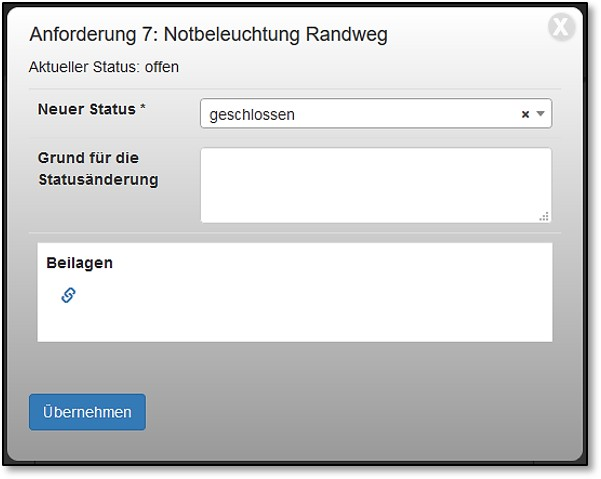
\includegraphics[width=0.5\linewidth]{../chapters/06_Anf-Maengelmanagement/pictures/amm_AnfStatusAendern.jpg}}
\caption{Status ändern}
% \label{fig:speciation}
\end{figure}

Bei der Statusänderung erscheint ein neues Fenster, in welchem man den nächstmöglichen Status auswählen kann. Zudem kann der Grund für die Statusänderung angegeben werden. \\

Auch bei einer Statusänderung kann ein Dokument verlinkt \col{(2)} werden, so zum Beispiel ein Foto als Nachweis.\\
\textbf{Hinweis:} Jedes Dokument, Foto etc, muss vorher in der Dokumentenablage erfasst werden, damit es hier zur Verfügung steht (Siehe Kapitel \ref{bkm:Ref442863508})

\begin{figure}[H]
\center{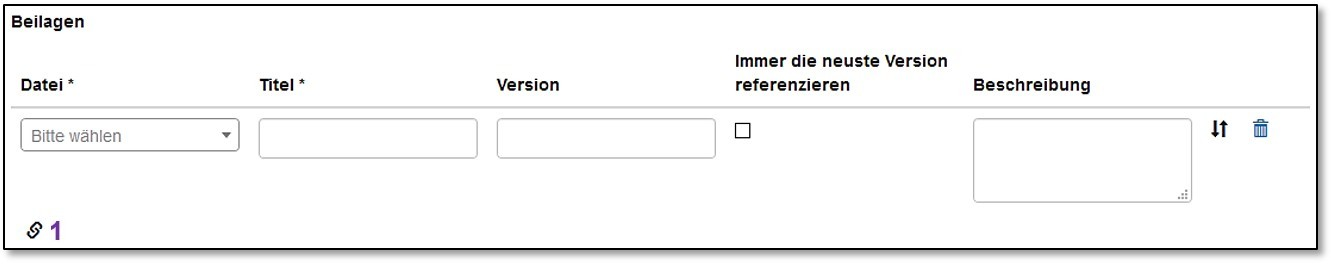
\includegraphics[width=1\linewidth]{../chapters/06_Anf-Maengelmanagement/pictures/amm_Status_Datei.jpg}}
\caption{Datei bei Statuswechsel verlinken}
% \label{fig:speciation}
\end{figure}

Danach geht die Kontrolle über den Status dieser Anforderung zur Prüfung an den TPL Validierung. 

\subsubsection{Erfassung abgeschlossen}

Der TPL Validierung überprüft, ob die Anforderung vollständig und korrekt erfasst wurde. Falls dies nicht der Fall ist, kann er entweder die Änderungen selbst durchführen oder den Status entsprechend zurücksetzen über die farbige Schaltfläche. Der TPL Validierung kann nun den Status auf 'Anforderung bearbeiten' zurücksetzen. Die Kontrolle geht dann wieder zum Ersteller. Ist die Anforderung korrekt und vollständig erfasst, kann der TPL Validierung den Status auf 'Erfassung abgeschlossen' setzen. \\

Am Ende einer RAMS-Phase sind alle Anforderungen idealerweise in diesem Status ('Erfassung abgeschlossen') und bleiben in diesem Zustand während der Ausführung. Vor dem Start zur Nachweisplanung, welche allenfalls Monate oder sogar Jahre später erfolgen kann, muss der TPL Validierung nochmals überprüfen, ob die Anforderungen immer noch korrekt sind. Wenn er selbst keine Änderungen anbringen möchte, setzt er entsprechend den Status entweder nochmals zurück auf 'Anforderung bearbeiten' oder weiter auf 'Nachweisplanung'. Im letzteren Fall liegt die Kontrolle über den Status dann beim Validierer der Anforderung, welcher die Nachweisplanung durchführt. 

\subsubsection{Nachweisplanung}
\label{bkm:Ref2018071811}

Der Validierer plant den Nachweis der Anforderung und füllt dazu bei der entsprechenden Maske 'Validierung der Anforderung (Planung)'  die einzelnen Felder aus. 

\begin{figure}[H]
\center{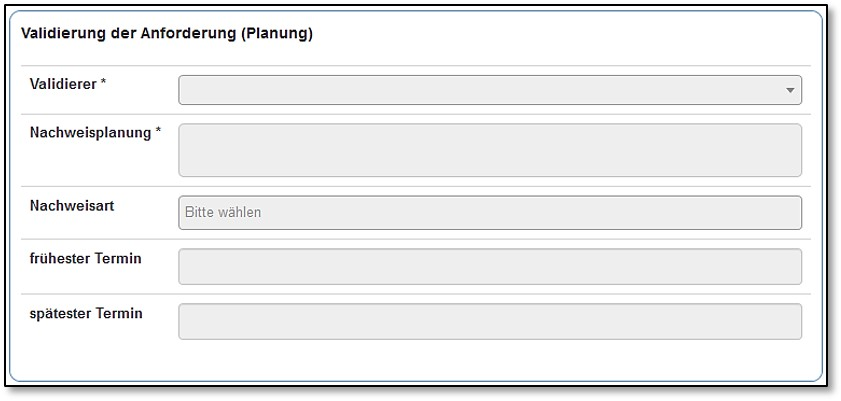
\includegraphics[width=.6\linewidth]{../chapters/06_Anf-Maengelmanagement/pictures/amm_ValidierungPlanung.jpg}}
\caption{Validierung der Anforderung}
% \label{fig:speciation}
\end{figure}

Nach dem 'Übernehmen' der Änderungen kann der Validierer den Status weiterschalten zu 'Nachweisplanung abgeschlossen'. Die Kontrolle über den Status obliegt nun wieder dem TPL Validierung zur Überprüfung der Planung. 

\subsubsection{Überprüfung der Nachweisplanung}

Der TPL Validierung überprüft, ob die Nachweisplanung vollständig und korrekt erfasst wurde. Falls dies nicht der Fall ist, kann er entweder die Änderungen selbst durchführen oder den Status entsprechend zurücksetzen über die farbige Schaltfläche. Der TPL Validierung hat nun die Möglichkeit den Status auf 'Nachweisplanung' zurückzusetzen. Die Kontrolle geht dann wieder zum Validierer. Ist die Nachweisplanung korrekt und vollständig, kann der TPL Validierung den Status auf 'Freigegeben zur Validierung' setzen. 

\subsubsection{Freigegeben zur Validierung - Planung}

Der Validierer erbringt den Nachweis zur Erfüllung der Anforderung selbst oder durch einen Drittanbieter und füllt dazu bei der entsprechenden Maske 'Validierung der Anforderung (Durchführung)' die einzelnen Felder aus. 

\begin{figure}[H]
\center{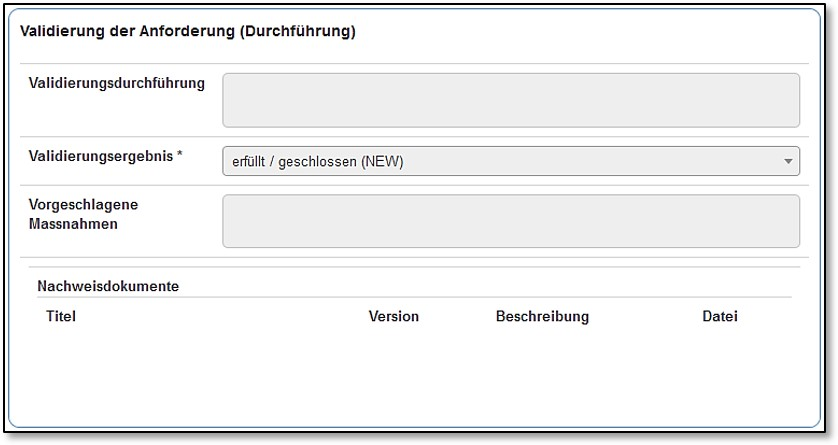
\includegraphics[width=.6\linewidth]{../chapters/06_Anf-Maengelmanagement/pictures/amm_ValidierungDurchf.jpg}}
\caption{Validierung der Anforderung - Durchführung}
% \label{fig:speciation}
\end{figure}

Wichtig ist dabei, dass er auch die entsprechenden Nachweisdokumente hinterlegt. Beim Validierungsergebnis wählt er gezielt aus einer der möglichen Endzustände für die Anforderung aus. Beinhaltet das Validierungsergebnis eine Massnahme, ist ein entsprechender Vorschlag im nächsten Feld zu formulieren. \\
 
Nach dem 'Übernehmen' der Änderungen kann der Validierer den Status im erscheinenden Fenster zu 'Überprüfung der Validierung' weiterschalten. Die Kontrolle über den Status obliegt nun wieder dem TPL Validierung zur Überprüfung der Validierung und Beurteilung des Validierungsergebnisses. 

\subsubsection{Überprüfung der Validierung}
\label{bkm:Ref2018071812}

Der TPL Validierung überprüft, ob die Durchführung der Validierung vollständig und korrekt erfasst wurde. Falls dies nicht der Fall ist, kann er entweder die Änderungen selbst durchführen oder den Status entsprechend über die farbige Schaltfläche zurücksetzen: 

\begin{figure}[H]
\center{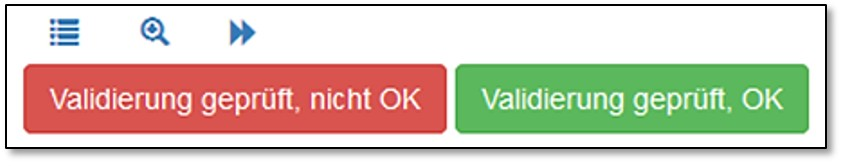
\includegraphics[width=0.5\linewidth]{../chapters/06_Anf-Maengelmanagement/pictures/amm_Ueberpruefung.jpg}}
\caption{Validierung überprüfen}
% \label{fig:speciation}
\end{figure}

Nun kann der TPL Validierung im Bedarfsfall den Status auf 'Freigegeben zur Validierung' zurücksetzen. Die Kontrolle geht dann wieder zum Validierer. Ist die Durchführung der Validierung korrekt und vollständig, kann der TPL Validierung den Status auf 'Validierung abgeschlossen' setzen. 

\subsubsection{Validierung abgeschlossen}

Der Validierungsprozess für diese Anforderung ist in diesem Status abgeschlossen. Das heisst nicht, dass die Anforderung zwingend erfüllt wurde. Es ist möglich, dass die Anforderung nicht erfüllt ist und weitere Massnahmen, z.B. betriebliche Massnahmen, notwendig sind. Die Erfassung von Massnahmen ist separat durchzuführen.

%% Kann/wird eine solche Massnahme mit einem anderen Modul abgedeckt -> Arbeitspaket, Mangel?

%bishierher

% \pagebreak

\subsection{Mängel (Vorbehalte)}

In Bezug auf die Anforderungen werden sämtliche Mängel erfasst. 

\begin{figure}[H]
\center{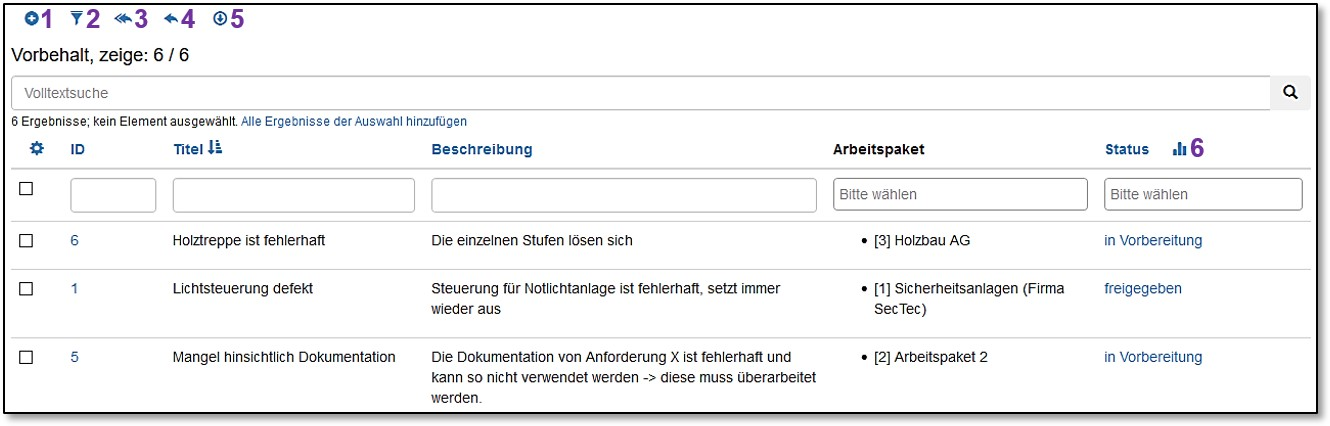
\includegraphics[width=1\linewidth]{../chapters/06_Anf-Maengelmanagement/pictures/amm_MaengelUebersicht.jpg}}
\caption{Übersicht der erfassten Mängel / Vorbehalte}
% \label{fig:speciation}
\end{figure}

\textbf{Die Mängelübersicht kurz erklärt:}

\vspace{\baselineskip}

\begin{compactitem}
	\item Mit dem Plussymbol (
\includegraphics[height=12pt]{/Icons/Plussymbol.jpg}) wird ein neuer Mangel erfasst. 
	\item Für die Suche bereits erfasster Mängel stehen wie gewohnt die Volltextsuche und die Spaltenfilterung zur Verfügung. Mit dem Filter-Symbol (
\includegraphics[height=12pt]{/Icons/Filter.jpg}) können Sie die erweiterten Filteroptionen einblenden (Such- und Filtereinstellungen speichern).
	\item Mit dem 
\includegraphics[height=12pt]{/Icons/Doppelpfeil_l.jpg}-Symbol können Sie sich alle Pendenzen anzeigen lassen, welche via Arbeitspaketen mit den ausgewählten Mängel verknüpft sind.
	\item Mit dem 
\includegraphics[height=12pt]{/Icons/Pfeil_l.jpg}-Symbol werden Ihnen alle Arbeitspakete angezeigt, welche mit den ausgewählten Mängel verknüpft sind.
	\item Mit dem 
\includegraphics[height=12pt]{/Icons/ListeGenerieren.jpg}-Symbol wird von den ausgewählten / gefilterten Mängel eine Excelliste erstellt.
\end{compactitem}

\vspace{\baselineskip}

Mit Klick auf die ID-Nummer eines Mangels können Sie den Mangel anzeigen lassen oder bearbeiten. Die Mängel besitzen ein Statussystem, welches den Zustand / Fortschritt der Bearbeitung dokumentiert. Mit Klick auf das Status-Symbol (
\includegraphics[height=12pt]{/Icons/Status.jpg}) erhalten Sie eine Statistik über den 'Zustand' der Mängel (Wie viele Mängel haben welchen Status).

\begin{figure}[H]
\center{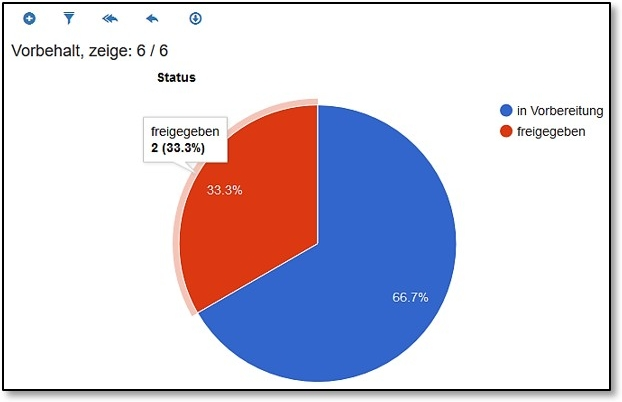
\includegraphics[width=.5\linewidth]{../chapters/06_Anf-Maengelmanagement/pictures/amm_MaengelStatistik.jpg}}
\caption{Visualisierung Statusübersicht der Mängel}
% \label{fig:speciation}
\end{figure}

\textbf{Neuen Mangel erfassen}

\begin{figure}[H]
\center{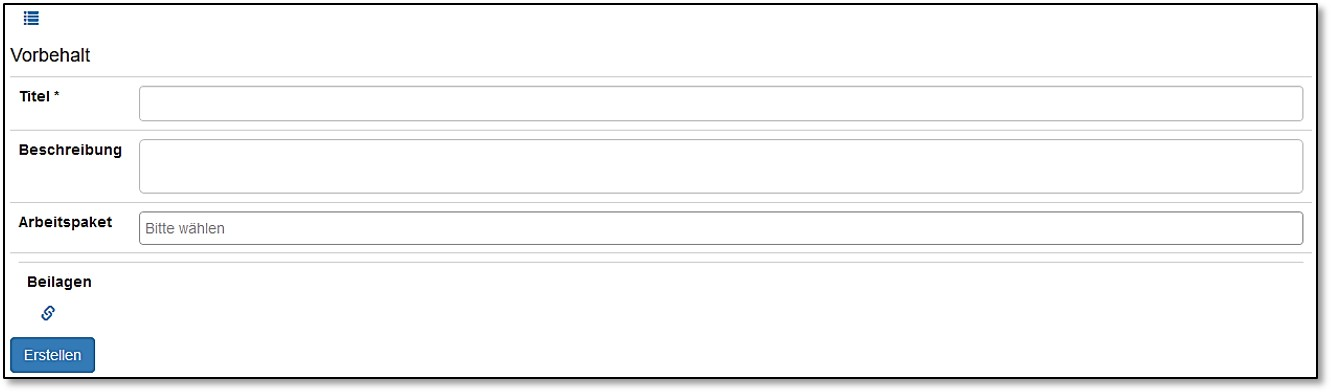
\includegraphics[width=1\linewidth]{../chapters/06_Anf-Maengelmanagement/pictures/amm_MaengelErfassen.jpg}}
\caption{Neuer Mangel erfassen}
% \label{fig:speciation}
\end{figure}

Geben Sie einen Titel (Pflichtfeld) und eine Beschreibung für den Mangel ein. Weiter kann der Mangel mit einem Arbeitspaket und einer Datei verknüpft werden (die gewünschte Datei muss vorher in der Dokumentenablage erfasst werden).\\
Nach Klick auf 'Erstellen' sind die Daten gespeichert und der neue Mangel angelegt. Mit dem Listensymbol (
\includegraphics[height=12pt]{/Icons/Listensymbol_zurueck.jpg}) gelangen Sie wieder zur Übersicht.

\vspace{\baselineskip}

\textbf{Tipp:} Wollen Sie nach dem Erstellen oder Bearbeiten eines Mangels (Vorbehaltes) direkt zur Übersicht zurückkehren, klicken Sie den Button 
\includegraphics[height=14pt]{/Icons/ueb_schliessen.png} oben in der Mitte des Bildschirms.

\vspace{\baselineskip}

\textbf{Hinweis:} Sie können bei den Vorbehalten Checklisten verknüpfen, welche Sie dann auch gleich von hier aus validieren können. Mehr zum Thema Checklisten finden Sie in Kapitel \ref{bkm:Ref2018102501}.

\pagebreak
\subsection{Arbeitspaket}

Arbeitspakete entsprechen einer Sammlung thematisch ähnlicher Mängel oder Pendenzen. Es enthält so zum Beispiel sämtliche Mängel, welche dann an Firma X zur Korrektur übergeben werden.

\begin{figure}[H]
\center{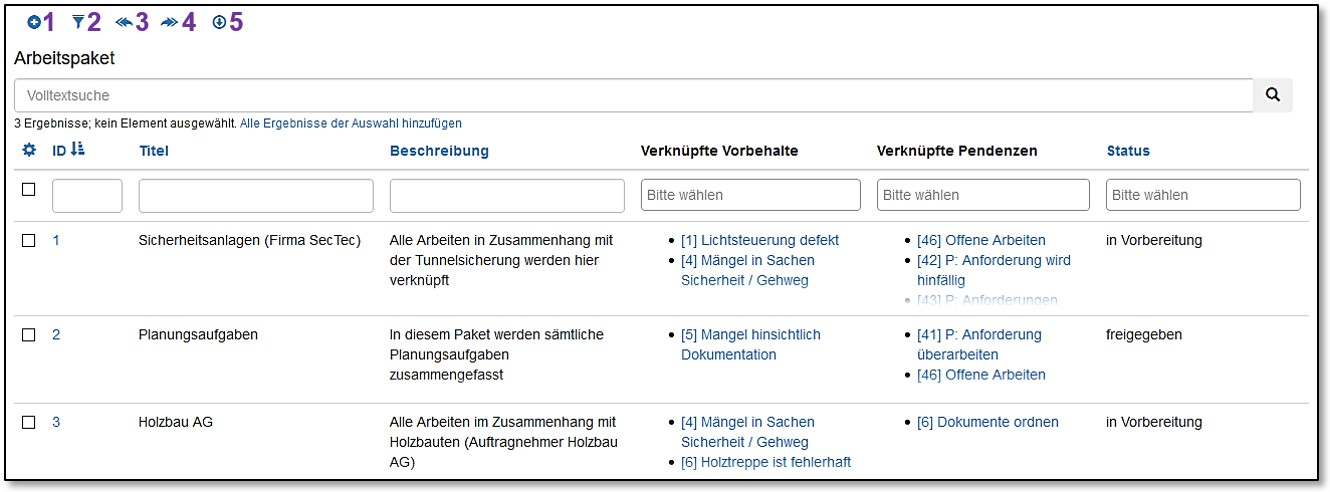
\includegraphics[width=1\linewidth]{../chapters/06_Anf-Maengelmanagement/pictures/amm_ArbeitspUebersicht.jpg}}
\caption{Übersicht der erfassten Arbeitspaketen}
% \label{fig:speciation}
\end{figure}

\textbf{Die Arbeitspaketübersicht kurz erklärt:}

\vspace{\baselineskip}

\begin{compactitem}
	\item Mit dem Plussymbol (
\includegraphics[height=12pt]{/Icons/Plussymbol.jpg}) wird ein neues Arbeitspaket erfasst. 
	\item Für die Suche bereits erfasster Arbeitspakete stehen wie gewohnt die Volltextsuche und die Spaltenfilterung zur Verfügung. Mit dem Filter-Symbol (
\includegraphics[height=12pt]{/Icons/Filter.jpg}) können Sie die erweiterten Filteroptionen einblenden (Such- und Filtereinstellungen speichern).
	\item Mit dem 
\includegraphics[height=12pt]{/Icons/Doppelpfeil_l.jpg}-Symbol können Sie sich alle Pendenzen anzeigen lassen, welche mit den ausgewählten Arbeitspaketen verknüpft sind.
	\item Mit dem 
\includegraphics[height=12pt]{/Icons/Doppelpfeil.jpg}-Symbol werden Ihnen alle Mängel angezeigt, welche mit den ausgewählten Arbeitspaketen verknüpft sind.
	\item Mit dem 
\includegraphics[height=12pt]{/Icons/ListeGenerieren.jpg}-Symbol wird von den ausgewählten / gefilterten Arbeitspaketen eine Excelliste erstellt.
\end{compactitem}

\vspace{\baselineskip}

Mit Klick auf die ID-Nummer eines Arbeitspakets können Sie den Arbeitspaket anzeigen lassen oder bearbeiten. Die Arbeitspakete besitzen ein Statussystem, welches den Zustand / Fortschritt der Bearbeitung dokumentiert.

\vspace{\baselineskip}

Bei den Spalten 'Verknüpfte Mängel / Verknüpfte Pendenzen' gelangen Sie mittels den blauen Titel (Links) direkt auf den entsprechenden Mangel, resp. die entsprechende Pendenz.

\pagebreak
\textbf{Ein neues Arbeitspaket erfassen:}

\begin{figure}[H]
\center{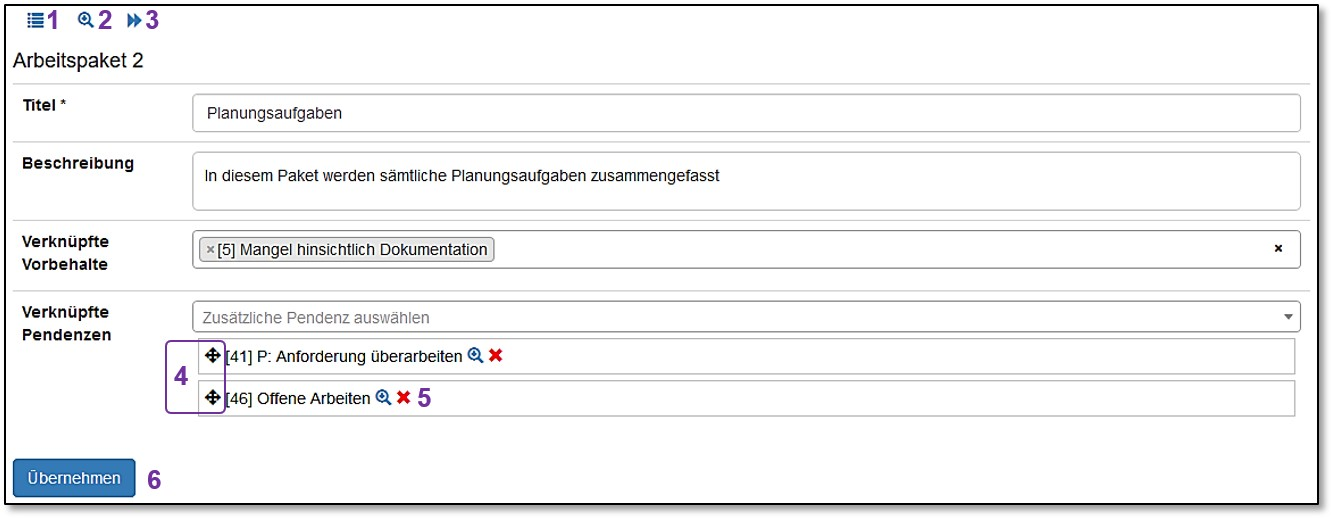
\includegraphics[width=1\linewidth]{../chapters/06_Anf-Maengelmanagement/pictures/amm_ArbeitspErstellen.jpg}}
\caption{Ein neues Arbeitspaket erstellen}
% \label{fig:speciation}
\end{figure}

Geben Sie für das Arbeitspaket einen aussagekräftigen Titel (Pflichtfeld) und eine Beschreibung ein.\\
Das Arbeitspaket kann bei 'Verknüpfte Mängel / Verknüpfte Pendenzen' mit Mängel, resp. Pendenzen verknüpft werden (Mehrfachauswahl). Mit dem 
\includegraphics[height=12pt]{/Icons/verschieben.jpg}-Symbol \col{(4)} können Sie die Reihenfolge der Pendenzen verändern. Packen Sie das Symbol und ziehen Sie die Zeile an die gewünschte Position. Mit dem Lupensymbol (
\includegraphics[height=12pt]{/Icons/Lupe.jpg}) \col{(5)} können Sie die Pendenz betrachten (Die Pendenz wird in neuem Browserfenster geöffnet). Mit dem roten Kreuzchen (
\includegraphics[height=12pt]{/Icons/roKreuzchen.jpg}) kann eine verknüpfte Pendenz wieder entfernt werden \col{(5)}. Speichern Sie die Eingaben mit Klick auf 'Übernehmen' \col{(6)}.

\vspace{\baselineskip}

Mit dem Listensymbol (
\includegraphics[height=12pt]{/Icons/Listensymbol_zurueck.jpg}) \col{(1)} gelangen Sie wieder zur Arbeitspaket-Übersicht. Mit dem Lupensymbol (\includegraphics[height=12pt]{/Icons/Lupe.jpg}) \col{(2)} können Sie das Arbeitspaket im Ansichtsmodus betrachten. Mit dem \includegraphics[height=12pt]{/Icons/Status_aendern.jpg}-Symbol \col{(3)} kann der Status verändert werden:

\begin{figure}[H]
\center{\includegraphics[width=.5\linewidth]{../chapters/06_Anf-Maengelmanagement/pictures/amm_ArbeitspStatus.jpg}}
\caption{Ein neues Arbeitspaket erstellen}
% \label{fig:speciation}
\end{figure}

In der Maske wird der mögliche neue Status vorgeschlagen. Geben Sie optional einen Grund für die Statusänderung ein und verknüpfen Sie bei Bedarf ein Dokument aus der Dokumentenablage (das gewünschte Dokument muss vorher in der Dokumentenablage hochgeladen werden).\\
Mit 'Übernehmen' werden die Eingaben gespeichert und der Vorgang abgeschlossen, mit dem Kreuzchen (\includegraphics[height=12pt]{/Icons/X_Button.jpg}) oben links verlassen Sie das Statusfenster ohne etwas zu speichern (Abbrechen).

\subsection{Pendenzen}

Für die Beauftragung von Validierungstätigkeiten kann die Pendenzen-Funktionalität genutzt werden. Dies ermöglicht es, Aufgaben bestimmten Einzelpersonen (z.B. Validierer) oder ganzen Gruppen (z.B. alle TPL Validierung) zuzuweisen. In der Regel reichen aber die Prozessschritte bei der Anforderungserfassung und -validierung geleitet durch den TPL Validierung aus. Die 'Pendenzübersicht' gibt den Erstellern und Validierern eine Auflistung aller pendenten Arbeitsschritte. 

\begin{figure}[H]
\center{\includegraphics[width=1\linewidth]{../chapters/06_Anf-Maengelmanagement/pictures/amm_PendUebersicht.jpg}}
\caption{Übersicht der Pendenzen}
% \label{fig:speciation}
\end{figure}

\textbf{Hinweis:} Bei den Pendenzen innerhalb des Anforderungs- und Mängelmanagement handelt es sich um das gleiche Modul wie bei den Pendenzen im Sitzungswesen. Entsprechend können Pendenzen mit Traktanden (Sitzungswesen) und Anforderungen, Arbeitspakete (Anforderungs- und Mängelmanagement) verknüpft werden. Mehr zu Pendenzen finden Sie in Kapitel \ref{bkm:Ref2018071802}.







